\section{SQL Injection Attack}

Gli attacchi di tipo SQL Injection sono una delle minacce alla sicurezza diffuse
e pericolose. Questo attacco si basa sull'invio di dati contenenti una
parte di query malevola per l'estrazione, modifica o cancellazione di tutti i
dati presenti all'interno di un database fruibile tramite un'applicazione web.

\begin{figure}[H]
    \centering
    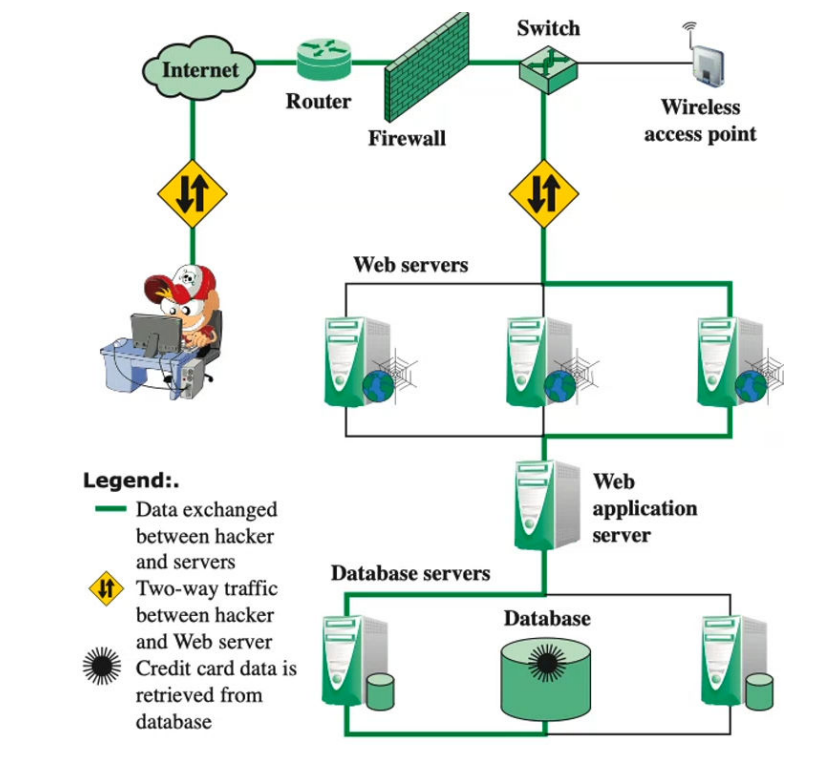
\includegraphics[width=10cm, keepaspectratio]{capitoli/sql_security/imgs/sql1.png}
    \caption{Esempio di un tipico attacco SQL Injection.}
\end{figure}

Questo attacco funziona tipicamente terminando prematuramente una stringa di
testo, generalmente con un commento \verb|--|, e aggiungendo un nuovo comando
che verrà eseguito dal database ed impedirà l'esecuzione del resto della query.\\

Possiamo caratterizzare gli attacchi SQL Injection in termini di via d'attacco e
tipo di attacco.

\subsection{Attack Avenues}

\begin{figure}[H]
    \centering
    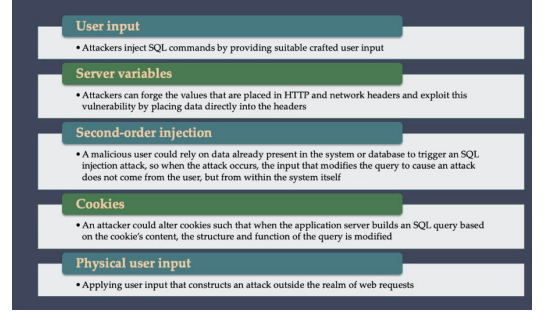
\includegraphics[width=10cm, keepaspectratio]{capitoli/sql_security/imgs/sql3.png}
\end{figure}

Le principali vie d'attacco sono le seguenti:

\paragraph{Input dell'utente:}
l'aggressore fornisce al database un input opportunamente modificato per
forzare l'esecuzione di una query malevola.

\paragraph{Variabili server:}
Le variabili del server sono un insieme di variabili che contengono intestazioni
HTTP, intestazioni del protocollo di rete e variabili ambientali. Le
applicazioni web usano queste variabili del server in una varietà di modi, come
la registrazione di statistiche e informazioni di utilizzo per identificare le
tendenze di un utente. Se queste variabili sono registrate in un database senza
sanificazione, questo potrebbe creare una vulnerabilità di SQL injection in
quanto è possibile modificarle ed inserirci codice arbitrario.

\paragraph{Second Order Injection:}
Un attaccante può sfruttare dati già presenti nel sistema o nel database per
attivare un attacco SQL Injection cosicché quando avviene effettivamente
l'attacco la query malevola non proviene dall'utente ma direttamente dal sistema
stesso.

\paragraph{Cookie:}
Di solito vengono utilizzati anche i cookie per creare in modo automatico query
per salvare dati o manipolarli. Un attaccante può modificare il contenuto di un
cookie per andare a forzare l'esecuzione di una query maligna all'interno di un
database.

\paragraph{Input fisico dell'utente:}
Gli attacchi SQL Injection possono anche avvenire all'esterno di una richiesta
web: prendiamo in considerazione un sistema che in automatico scannerizza e
archivia documenti tramite l'ausilio di modelli di machine learning, questo può
essere attaccato scrivendo fisicamente una query malvagia all'interno del
documento da acquisire.


\subsection{Attack Types}

I tipi di attacco possono essere raggruppati in tre categorie principali:
\textbf{In-band}, \textbf{Inferential}, \textbf{Out of Band}.

\paragraph{In-Band.}
Un attacco in banda utilizza lo stesso canale di comunicazione per iniettare
codice SQL e recuperare i risultati. I dati recuperati sono presentati
direttamente nella pagina web dell'applicazione. I tipi di attacco In-Band
includono i seguenti:

\begin{itemize}
    \item \textbf{Tautologia}: Questa forma di attacco inietta codice in una o
          più dichiarazioni condizionali in modo che valutino sempre vero.
    \item \textbf{Commento di fine riga}: Dopo aver iniettato codice in un
          particolare campo, il codice legittimo che segue viene annullato
          attraverso l'uso di commenti di fine riga. Un esempio potrebbe
          essere quello di aggiungere "\verb|--|" dopo gli input in modo che
          le query rimanenti non siano trattate come codice eseguibile, ma come
          commenti.
    \item \textbf{Query piggybacked}: L'attaccante riesce ad aggiunge ed
          eseguire ulteriori query oltre a quella originale. Questa
          tecnica si basa su configurazioni del server che permettono diverse
          query all'interno di una singola stringa di codice.
\end{itemize}

\paragraph{Inferential.}
Sono attacchi che non fanno trasferimento dei dati, quindi sono attacchi su
confidenzialità e non integrità. L'attaccante è in
grado di ricostruire le informazioni e risalire a specifiche segrete del database
inviando particolari richieste
e osservando il comportamento risultante del server.
Le principali metodologie di attacco sono:
\begin{itemize}
    \item \textbf{Query illegali/logicamente scorrette:} La vulnerabilità
          sfruttata da questo metodo è che la pagina di errore
          predefinita restituita dai server delle applicazioni è
          spesso eccessivamente descrittiva. Infatti, il semplice
          fatto che viene generato un messaggio di errore può
          spesso rivelare parametri vulnerabili per un
          attaccante.

    \item \textbf{Blind SQL Injection:} Permette agli attaccanti di dedurre i
          dati presenti in un sistema di database anche quando il sistema è
          sufficientemente sicuro da non mostrare alcuna informazione errata
          all'attaccante.
\end{itemize}

\paragraph*{Out-of-band.}
Sono degli attacchi in cui l'input dell'attacco avviene per un canale e l'output
per un altro canale. In un attacco fuori banda, i dati vengono recuperati
utilizzando un canale diverso, ad esempio una e-mail con i risultati della query
viene generata e inviata all'attaccante. Questo può essere utilizzato quando ci
sono limitazioni sul recupero delle informazioni, ma la connettività in uscita
dal server del database non presenta importanti restrizioni.\footnote{Questo
    concetto è finemente espresso con la seguente parola: \textit{lassista}
    \emoji{teacher-light-skin-tone}.}
